\chapter{Background}
\label{ch:background}

This chapter introduces the formal foundations underlying the IVM$^+$ approach and the adjusted variant studied in this thesis.
We first fix our data model and the class of queries we study, and introduce a running example that we revisit throughout the thesis (Section~\ref{sec:queries}).
We then introduce tree decompositions (Section~\ref{sec:tree_decompositions}), the structure the IVM$^+$ approach is organized around, and the fractional hypertree width derived from them (Section~\ref{sec:fhw}).

\section{Data Model and Queries}
\label{sec:queries}

We use standard relational terminology, which we briefly recall here~\cite{abiteboul1995}.

\medskip

A \emph{relation} $R$ is a finite set of tuples, and a \emph{database} $\mathcal{D}$ is a finite set of relations.
The \emph{size} $|R|$ of a relation is its number of tuples, and the size $|\mathcal{D}|$ of a database is the sum of the sizes of its relations.

\medskip

A \emph{full conjunctive query}, also called a \emph{natural join query}~\cite{abokhamis2024Insert-Only}, has the form
\[
Q = R_1(\mathbf{X}_1) \bowtie \cdots \bowtie R_k(\mathbf{X}_k),
\] 
where each $R_i$ is a relation symbol and each $\mathbf{X}_i$ is a tuple of variables, the \emph{schema} of $R_i$. Each $R_i(\mathbf{X}_i)$ is an \emph{atom} of $Q$, and $\mathrm{vars}(Q) = \bigcup_{i=1}^{k} \mathbf{X}_i$ denotes the set of all variables of $Q$.
We call such a query \emph{full} because every variable in $\mathrm{vars}(Q)$ is returned in the result; no variables are projected away.
For brevity we refer to full conjunctive queries simply as \emph{queries}.

A tuple $t$ over $\mathrm{vars}(Q)$ is in the \emph{result} $Q(\mathcal{D})$ if each atom $R_i(\mathbf{X}_i)$ can be matched to a tuple $t_i \in R_i$ so that the matched tuples agree on their shared variables: for every variable $x \in \mathrm{vars}(Q)$, all matched tuples $t_i$ with $x \in \mathbf{X}_i$ assign $x$ the same value, namely $t(x)$.
For a tuple $t$ and a variable $x$ in its schema, $t(x)$ denotes the value that $t$ assigns to $x$.

\paragraph{Running example.}
As a running example we use a small \emph{self-join} query over a single binary relation $E$, which we read as the edge set of a directed graph.
Consider
\[
Q_\diamond = E_1(A,B) \bowtie E_2(B,C) \bowtie E_3(C,D) \bowtie E_4(B,D) \bowtie E_5(A,D),
\]
with $\mathrm{vars}(Q_\diamond) = \{A,B,C,D\}$.
Here $E_1,\dots,E_5$ all denote the same relation $E$; we treat each atom as a distinct occurrence of $E$ over the same data, which is standard and does not affect the tree decompositions and widths defined in the following sections.
We examine its structure and tree decomposition in Section~\ref{sec:tree_decompositions} and determine its fractional hypertree width in Section~\ref{sec:fhw}; we return to $Q_\diamond$ throughout the thesis, including as a benchmark query in our experiments (Chapter~\ref{ch:evaluation}).

\section{Tree Decomposition}
\label{sec:tree_decompositions}

The structure of a query is captured by its \emph{hypergraph}: the vertices are the variables $\mathrm{vars}(Q)$, and each atom $R_i(\mathbf{X}_i)$ contributes a hyperedge on its variables $\mathbf{X}_i$.
When all atoms are binary, as in our running example, the hypergraph is an ordinary undirected graph.
For $Q_\diamond$ it is the \emph{diamond} shown in Figure~\ref{fig:diamond_hypergraph}: two triangles $\{A,B,D\}$ and $\{B,C,D\}$ sharing the edge $B\text{--}D$.

\begin{figure}[ht]
  \centering
  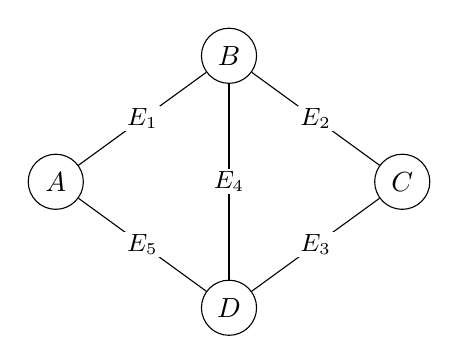
\begin{tikzpicture}[
    vertex/.style={circle, draw, minimum size=7mm, inner sep=0pt},
    lbl/.style={midway, font=\small, fill=white, inner sep=1pt}]
    \node[vertex] (B) at (0,1.6)  {$B$};
    \node[vertex] (D) at (0,-1.6) {$D$};
    \node[vertex] (A) at (-2.2,0) {$A$};
    \node[vertex] (C) at (2.2,0)  {$C$};
    \draw (A) -- (B) node[lbl] {$E_1$};
    \draw (B) -- (C) node[lbl] {$E_2$};
    \draw (C) -- (D) node[lbl] {$E_3$};
    \draw (B) -- (D) node[lbl] {$E_4$};
    \draw (A) -- (D) node[lbl] {$E_5$};
  \end{tikzpicture}
  \caption{The hypergraph of $Q_\diamond$.}
  \label{fig:diamond_hypergraph}
\end{figure}

\medskip

A \emph{tree decomposition}~\cite{cygan2015} $(\mathcal{T}, \chi)$ of a query $Q = R_1(\mathbf{X}_1) \bowtie \cdots \bowtie R_k(\mathbf{X}_k)$ consists of a rooted tree $\mathcal{T}$, whose nodes are called \emph{bags}, together with a function $\chi$ that assigns each bag $b$ a set of variables $\chi(b)$.
A valid tree decomposition satisfies two conditions:

\begin{enumerate}
    \item \textbf{Coverage:} Every atom $R_i(\mathbf{X}_i)$ is assigned to at least one bag $b$ with $\mathbf{X}_i \subseteq \chi(b)$.
    \item \textbf{Connectivity:} For every variable $x \in \mathrm{vars}(Q)$, the set of bags $\{b \mid x \in \chi(b)\}$ forms a connected subtree of $\mathcal{T}$.
\end{enumerate}

\paragraph{Running example.}
Figure~\ref{fig:diamond_td} shows a tree decomposition of $Q_\diamond$. It has two bags, one for each triangle of the hypergraph (Figure~\ref{fig:diamond_hypergraph}):
\begin{itemize}
    \item the root bag $b_1 = \{A, B, D\}$, covering the atoms $E_1(A,B)$, $E_4(B,D)$, and $E_5(A,D)$;
    \item the child bag $b_2 = \{B, C, D\}$, covering the atoms $E_2(B,C)$, $E_3(C,D)$, and $E_4(B,D)$.
\end{itemize}
Both conditions hold: every atom is covered, with the shared atom $E_4(B,D)$ lying in both bags, and every variable induces a connected subtree, since $A$ and $C$ each occur in a single bag while $B$ and $D$ occur in the two adjacent bags.
This is one of several valid tree decompositions of $Q_\diamond$; Section~\ref{sec:fhw} makes precise how their quality is measured.

\begin{figure}[ht]
  \centering
  \begin{tikzpicture}[bag/.style={draw, ellipse, minimum width=24mm, minimum height=11mm, inner sep=2pt}]
    \node[bag, label={[font=\small]left:$b_1$}] (r) at (0,1.9) {$\{A,B,D\}$};
    \node[bag, label={[font=\small]left:$b_2$}] (c) at (0,0)   {$\{B,C,D\}$};
    \draw (r) -- (c);
  \end{tikzpicture}
  \caption{A tree decomposition of $Q_\diamond$.}
  \label{fig:diamond_td}
\end{figure}

\section{Fractional Hypertree Width}
\label{sec:fhw}

Let $\mathbf{V} \subseteq \mathrm{vars}(Q)$.
A \emph{fractional edge cover}~\cite{atserias2013} of $\mathbf{V}$ assigns a weight $\lambda_i \in [0,1]$ to each atom $R_i(\mathbf{X}_i)$ of $Q$ so that every variable in $\mathbf{V}$ is covered, i.e.\ the weights of the atoms whose schema contains it sum to at least one.
The \emph{fractional edge cover number} $\rho^\ast(\mathbf{V})$ is the smallest total weight of such a cover:
\[
\begin{array}{@{}ll@{\qquad}l@{}}
\text{min}   & \displaystyle \sum\nolimits_{i=1}^{k} \lambda_i & \\[8pt]
\text{s.t.} & \displaystyle \sum\nolimits_{i\,:\, x \in \mathbf{X}_i} \lambda_i \geq 1 & \forall\, x \in \mathbf{V}, \\[8pt]
                  & \lambda_i \in [0,1] & \forall\, i
\end{array}
\]
Intuitively, $\rho^\ast(\mathbf{V})$ is the least number of atoms needed to cover $\mathbf{V}$, with fractional weights allowed.

\medskip

The \emph{fractional hypertree width}~\cite{grohe2014} $w(Q)$ of $Q$ is the smallest value, over all tree decompositions $(\mathcal{T}, \chi)$, of the largest fractional edge cover number $\rho^\ast(\chi(b))$ among the bags $b$ of $\mathcal{T}$:
\[
w(Q) = \min_{(\mathcal{T}, \chi)} \; \max_{b \in \mathcal{T}} \; \rho^\ast(\chi(b)).
\]
In particular, a tree decomposition with a single bag has that bag equal to $\mathrm{vars}(Q)$, so the maximum over its bags is just $\rho^\ast(\mathrm{vars}(Q))$; since $w(Q)$ minimizes over all tree decompositions, $w(Q) \le \rho^\ast(\mathrm{vars}(Q))$.

\paragraph{Running example.}
The single-bag decomposition has $\rho^\ast(\{A,B,C,D\}) = 2$: giving $E_1(A,B)$ and $E_3(C,D)$ weight $1$ each covers all four variables, and no cover is lighter.
The two-triangle decomposition of Figure~\ref{fig:diamond_td} does better: in each triangle bag, weight $\tfrac12$ on each of its three edges covers its three variables, so $\rho^\ast(\chi(b)) = \tfrac{3}{2}$ for both bags.
No tree decomposition can do better, hence $w(Q_\diamond) = \tfrac{3}{2} < 2$.

\medskip

The IVM$^+$ approach is built on a tree decomposition of minimum fractional hypertree width, which governs the cost of maintaining the query~\cite{abokhamis2024Insert-Only}.
Computing such a decomposition is NP-hard~\cite{fischl2018}, and approximation algorithms exist~\cite{marx2010}.
Our decomposer instead uses a practical heuristic: it generates candidate decompositions with a Minimum Fill-in heuristic~\cite{bodlaender2005} and selects the one of least fractional hypertree width, as described in more detail in Chapter~\ref{ch:implementation}.

